% !TeX program = pdflatex
% QRNG_Experiments_Phase_I_Phase_II_Report_2026.tex
% Phase I and Phase II QRNG experiments: closure report for ToE corpus and Overleaf.

\documentclass[reprint,amsmath,amssymb,aps,showkeys]{revtex4-2}
\usepackage[T1]{fontenc}
\usepackage[utf8]{inputenc}
\usepackage{lmodern}
\usepackage{microtype}
\usepackage{graphicx}
\usepackage{booktabs}
\usepackage{enumitem}
\usepackage{siunitx}
\sisetup{
  detect-weight=true,
  detect-family=true,
  table-format=1.6
}
\usepackage{tikz}
\usetikzlibrary{positioning}
\usepackage{hyperref}
\hypersetup{colorlinks=true,linkcolor=blue,citecolor=blue,urlcolor=blue}

\title{QRNG Experiments: Phase I and Phase II Closure Report\\
ANU Quantum Random Numbers, Intervention and Swarm Pilots}

\author{C.~M.~Baird}
\affiliation{Baird--ZoraASI Collaboration}

\date{March 2026}

\begin{document}
\maketitle

\begin{abstract}
Phase I tested whether meditation (or focused ethical intention) during QRNG collection produces measurable deviation from standard quantum randomness, as suggested by the MQGT-SCF ethics-weighted collapse channel; Phase II tested exploratory swarm/coherence pilots at 100k bits. Both phases are closed: Phase I with a null result (pooled permutation $p = 0.41$); Phase II with non-replication of an exploratory hint (Pilot 3 did not replicate Pilot 2's directional ordering). The pipeline, statistical suite, and pre-specified decision rules were validated. Closure and follow-up are recorded in version control (commits \texttt{c5e6886}, \texttt{4c4d866}) for citation.
\end{abstract}

\noindent\textbf{Keywords:} quantum random number generator, hypothesis testing, replication, exploratory pilot, experimental closure.

\section{Introduction}

The MQGT-SCF framework allows for consciousness-related or ethics-weighted influence on quantum measurement outcomes. A testable prediction is that focused intention or coherent multi-agent states might bias the statistics of a quantum random number generator (QRNG). Phase I tested a single-intervention design (meditation during collection) using the ANU Quantum Random Numbers API; Phase II tested exploratory swarm/coherence pilots at 100k bits per run. Both phases are now formally closed: Phase I with a documented null; Phase II with a failed replication and protocol closure. This report transcribes the methods, results, decision rule, and conclusion for inclusion in the ToE corpus and Overleaf.

\section{Methods}

\subsection{Phase I}
Random numbers were obtained from the Australian National University Quantum Random Number Generator (ANU QRNG), which derives randomness from vacuum fluctuations of light. Phase I used a block-randomized design: control vs.\ intervention (meditation or focused ethical intention) during collection. Scale: 6 million bits total in three independent runs of 2M bits each (20 blocks $\times$ 100k bits per run). Block order was randomized with seeds 42, 123, and 456. A single ANU API endpoint was used with no fallback. Pipeline: ANU Quantum Random Numbers API $\to$ raw bits $\to$ block summaries $\to$ bias, runs, entropy, autocorrelation tests $\to$ permutation test on control vs.\ intervention block means (10,000 permutations).

\subsection{Phase II}
Phase II comprised exploratory pilots at 100k bits per pilot. Scale: 100k bits per pilot; single ANU endpoint, preflight, no fallback.
\begin{itemize}[noitemsep]
\item Pilot 0: Control only (10 blocks $\times$ 10k bits).
\item Pilot 1: Single-agent vs.\ control (5 control + 5 single-agent blocks, randomized).
\item Pilot 2: Swarm low vs.\ high (4 control + 3 swarm\_low + 3 swarm\_high blocks, randomized).
\item Pilot 3: Replicate 2 of Pilot 2---same design, block structure, endpoint, and pacing; new replicate ID only.
\end{itemize}

\section{Results}

\begin{figure}[h]
\centering
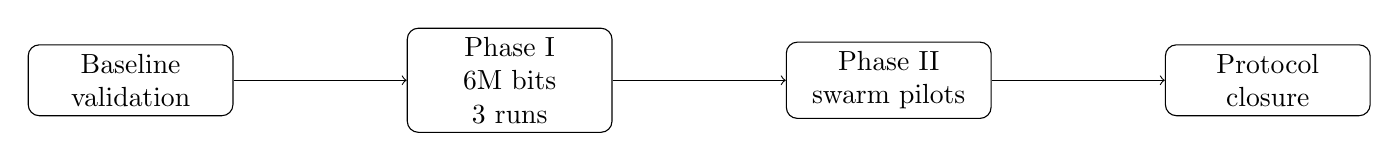
\begin{tikzpicture}[
    node distance=2.2cm,
    every node/.style={draw, rectangle, rounded corners, align=center, minimum width=2.6cm}
]
\node (baseline) {Baseline \\ validation};
\node (phase1) [right=2.2cm of baseline] {Phase I \\ 6M bits \\ 3 runs};
\node (phase2) [right=2.2cm of phase1] {Phase II \\ swarm pilots};
\node (closure) [right=2.2cm of phase2] {Protocol \\ closure};
\draw[->] (baseline) -- (phase1);
\draw[->] (phase1) -- (phase2);
\draw[->] (phase2) -- (closure);
\end{tikzpicture}
\caption{Timeline of the QRNG experiment sequence.}
\end{figure}

\subsection{Phase I}
Control and intervention blocks showed no statistically significant difference (pooled permutation $p = 0.41$). For $N = 6\times10^6$ bits, the expected standard deviation of the proportion of ones is approximately $\sigma \approx 2\times10^{-4}$, so the observed deviation ($\Delta \approx 3.3\times10^{-4}$) lies well within normal statistical fluctuation. Run 3 showed a sign flip (intervention slightly below control), as expected under the null.

\begin{table}[h]
\centering
\caption{Phase I QRNG intervention runs (6M bits total).}
\label{tab:phase1}
\begin{tabular}{l
  S[table-format=1.4]
  S[table-format=1.4]
  S[table-format=-1.5]
  S[table-format=1.2]}
\toprule
Run & {Control mean} & {Intervention mean} & {Difference} & {$p$} \\
\midrule
Seed 42  & 0.4997 & 0.5006 & 0.00094 & 0.17 \\
Seed 123 & 0.4996 & 0.5003 & 0.00069 & 0.37 \\
Seed 456 & 0.5004 & 0.4997 & -0.00064 & 0.28 \\
\midrule
Pooled   & 0.4997 & 0.5000 & 0.00033 & 0.41 \\
\bottomrule
\end{tabular}
\end{table}

\paragraph{Close-out statement.}
Phase I QRNG experiments (March 2026) collected 6 million bits across three independent intervention sessions using a block-randomized design. Control and intervention blocks showed no statistically significant difference (pooled permutation $p = 0.41$). Observed differences were consistent with binomial variation. The pipeline, statistical test suite, and replication protocol were validated. Phase I therefore concludes that no detectable effect was observed at the current sensitivity level. Interpretation: no detectable intervention effect was observed within the sensitivity limits of the experiment.

\subsection{Phase II}
Table~\ref{tab:phase2} gives condition means by pilot. Pilot 2 showed ordering swarm\_low $>$ control $>$ swarm\_high; Pilot 3 reversed to control $>$ swarm\_low $>$ swarm\_high.

\begin{table}[h]
\centering
\caption{Phase II exploratory swarm pilots (100k bits per pilot): proportion of ones by condition.}
\label{tab:phase2}
\begin{tabular}{l S[table-format=1.4] S[table-format=1.4] S[table-format=1.4]}
\toprule
Pilot & {Control} & {Swarm\_low} & {Swarm\_high} \\
\midrule
Pilot 0 & 0.5005 & \multicolumn{1}{c}{--} & \multicolumn{1}{c}{--} \\
Pilot 1 & 0.5010 & 0.4998 & \multicolumn{1}{c}{--} \\
Pilot 2 & 0.4989 & 0.5047 & 0.4985 \\
Pilot 3 & 0.5027 & 0.4978 & 0.4956 \\
\bottomrule
\end{tabular}
\end{table}
\noindent Pilot~3 reverses the exploratory ordering observed in Pilot~2, indicating that the apparent separation was consistent with random variation rather than a reproducible effect.

\section{Decision rule and closure}

\paragraph{Pre-specified rule.}
If Pilot 3 does not show the same directional ordering as Pilot 2, treat Pilot 2 as noise/artifact and do not scale. If Pilot 3 does show the same ordering, run Pilot 4 (replicate 3) before any escalation.

\paragraph{Outcome.}
Pilot 3 did not replicate Pilot 2. Per the rule: Pilot 4 was not run; no escalation to 1M or 10M. The 100k swarm pilot sequence is closed.

\paragraph{Conclusion.}
No reproducible swarm effect was detected at the 100k level. The Pilot 2 separation (swarm\_low $>$ control $>$ swarm\_high) is consistent with statistical noise or protocol artifacts. Phase II 100k exploratory pilot sequence is therefore closed.

\section{Discussion}

The exploratory swarm pilot initially produced a directional separation (Pilot 2), but this ordering failed replication in Pilot 3. Following the pre-specified decision rule, no further escalation was performed and the protocol was closed. The process followed sound experimental practice: baseline validation; exploratory pilot with defined conditions; replication before scaling; predefined decision rule; stopping when replication failed. The QRNG pipeline and experimental discipline were validated even though the hypothesis did not show an effect. If Phase II swarm/coherence work continues, the recommended next step is not to scale this protocol but to conduct a protocol audit (block synchronization timing, swarm state definition, agent independence, API batching, condition labeling) and design a new pilot protocol rather than scaling one that already failed replication.

\section{Data and code availability}

Artifacts (raw bits, summaries) reside in the TOE repository under \texttt{artifacts/}, which is gitignored; they are available on request or via Zenodo if deposited. No API keys or secrets are in the repository. Repository state corresponding to the closure of the QRNG branch is recorded on branch \texttt{main} at commits \texttt{c5e6886} (protocol closure) and \texttt{4c4d866} (protocol audit and lessons learned).

\section*{References}

Phase I full report, Phase II close-out, runbook, staged program, and method doc are in the TOE repository (docs/ and papers\_sources/). Canonical Zenodo: \url{https://doi.org/10.5281/zenodo.18792939}. Repository: \url{https://github.com/Cbaird26}.

\end{document}
